\documentclass[]{article}
\usepackage[T1]{fontenc}
\usepackage[utf8]{inputenc}
\usepackage[polish]{babel}
\usepackage{enumitem}
\usepackage{graphicx}

%\usepackage[top=1in, bottom=1in, left=1in, right=1in]{geometry}

\title{Phishing}
\author{Nikodem Kaczmarek, Patryk Garwol}

\begin{document}
\maketitle
\begin{figure}[h!]
	\centering
	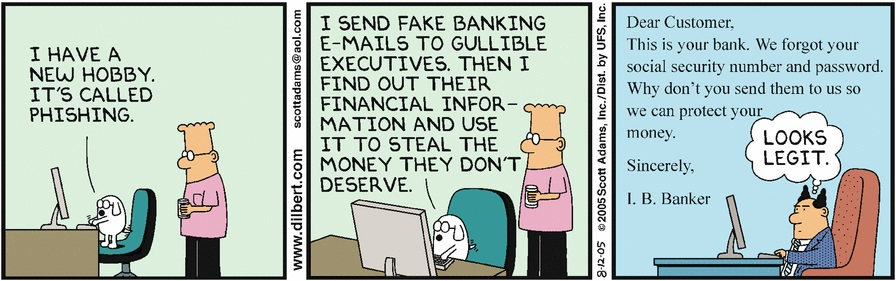
\includegraphics[width=\linewidth]{Pictures/phishing_comics.jpg}
	\caption{Humorystyczne ukazanie Phishingu, Scott Adams, 2005}
	\label{fig:pp_phishing2019}
\end{figure}


\newpage 

\section{Wprowadzenie}




\newpage
\section{Mechanizm działania phishingu}

Phishing przypomina słowo fishing, w szczególności gdy skupimy się na wymowie. Nie jest to przypadek, ponieważ ataki tego rodzaju są w pewien sposób "łowieniem rybek" \cite{govpl_phishing}:
\begin{itemize}[label=$\rightarrow$]
	\item wędkarz - przestępca
	\item przynęta - wiadomość, szkodliwy link, fałszywa strona itp.
	\item ryba - zasoby nieświadomej ofiary
\end{itemize} 

Mowa tutaj zatem o inżynierii społecznej, czyli technice manipulacji, która wykorzystuje ludzkie błędy w celu uzyskania prywatnych informacji lub innych zasobów \cite{kaspersky_social_engineering}.
Zdarzają się również przypadki, w których przestępca jest na tyle złośliwy, że wykorzystując phishing instaluje na sprzęcie ofiary złośliwe oprogramowanie, które niekoniecznie służy do kradzieży danych. Oszustwa te wykorzystują najsłabsze ogniwo w świecie informatyki, czyli człowieka. Większość populacji, w szczególności osoby starsze - nie jest obeznana w kwestii informatyki \cite{dsgi_wiley}, nie mówiąc już o cyberbezpieczeństwie. Łatwo jest wykorzystać ich niewiedzę, co w połączeniu z socjotechnikami daje atakującym dużo pola do popisu w kwestii doboru ich "przynęty".

Atak phishingowy może zostać przeprowadzony na nieokreślonych ofiarach. Atakujący wówczas liczą, że ktokolwiek "złapie się na haczyk". W dobie internetu bardzo łatwo jest wysyłać e-maile, lub nawet sms-y do niezliczonej liczby osób. Próg wejścia do zautomatyzowania takich procesów jest bardzo niski i ofiara nie potrzebuje lat nauki programowania, żeby do takiego ataku doprowadzić, ponieważ wystarczy zainstalować na komputerze IDE Pythona, a następnie poświęcić 5 sekund życia, aby znaleźć odpowiedni przewodnik, na przykład "How to Send Automated Email Messaged in Python" opublikowany w witrynie geeksforgeeks.org \cite{geeks4geeks_automaticmails}. Czyni to ten proceder bardziej przerażającym, wiedząc jak proste jest to przedsięwzięcie. Zdecydowana osób nie nabierze się na e-mail przysłowiowego Księcia z Nigerii \cite{nigerian_prince}. Jest jednak procent ludzi, które są podatne na ataki tego typu.

Groźniejszym rodzajem phishingu jest spear-phishing. Polega on na zaatakowaniu określonej osoby lub podmiotu, co rażąco wpływa na jego skuteczność. Ataki te są planowane dłuższy czas, aby dokładnie poznać słabe strony ofiary i tym sposobem zoptymalizować szanse powodzenia. Według raportu firmy Proofpoint z roku 2020, w roku 2019. 88\% organizacji na świecie doświadczyło zagrożenia tego rodzaju. Spośród nich aż 55\% stało się jego ofiarami \cite{proofpoint2020}.

\begin{figure}
	\centering
	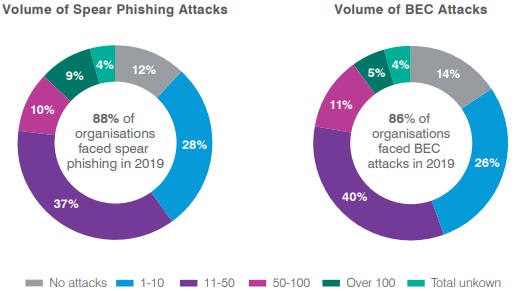
\includegraphics[width=0.8\linewidth]{Pictures/proofpoint_phishing2019.jpg}
	\caption{Skala ataków phishingowych w 2019. roku wg. raportu Proofpoint}
	\label{fig:pp_phishing2019}
\end{figure}

\newpage
\section{Wybrane narzędzia i techniki wykorzystywane przez oszustów}

\subsection{Inżynieria społeczna}
Inżynieria społeczna została już przez nas wspomniana. Nazwa jest dość enigmatyczna, aczkolwiek sprowadza się do relatywnie prostej rzeczy - oszukanie człowieka. Kilka sposobów na osiągnięcie tego efektu to:
\begin{itemize}[label=$\rightarrow$]
	\item Pretexting - opiera się na budowaniu zaufania. Wymyślane są przeróżne scenariusze, których atakujący używają do nakłonienia ofiar, aby ujawniły informacje. Przestępca może użyć pretekstu, aby podszyć się pod personel IT i poprosić o dane logowania.
	\item Podszywanie się pod kierownictwo - znane również jako CEO fraud, jest to połączenie spear-phishingu oraz pretextingu. Jak nazwa wskazuje, atakujący podszywa się pod przełożonego ofiary, przez co zdecydowanie łatwiej jest taką osobę nabrać .
	\item Romansowe oszustwa - oszuści wykorzystują aplikacje (stricte randkowe) w celu znalezienia ofiary, aby następnie budować z nią romantyczną relację i w odpowiednim momencie zaatakować \cite{abnormal_phishingtypes}.
\end{itemize} 

\subsection{Spoofing}
Spoofing odnosi się do fałszowania lub modyfikowania informacji w celu wprowadzenia w błąd lub oszukania odbiorcy co do prawdziwego źródła lub tożsamości nadawcy. Spoofing i phishing to de facto dwa różne sposoby ataku, jednakże często idą w parze. Warto tu nadmienić, że:
\begin{itemize}[label=$\rightarrow$]
	\item Atak spoofingowy {\bfseries może} utworzyć grunt pod atak phishingowy
	\item Atak phishingowy {\bfseries nigdy} nie tworzy gruntu pod atak spoofingowy
\end{itemize}
Choć różnica między tymi atakami może być na pierwszy rzut oka niejasna, sedno motywacji wyżej wymienioncyh działań jest zgoła odmienne. Celem spoofingu jest podszywanie się pod czyjąś tożsamość, podczas gdy celem ataków phishingowych jest kradzież informacji \cite{crowdstrike_phishing_vs_spoofing}.
Podszycie się może zostać osiągnięte na różne sposoby, m.in:
\begin{itemize}[label=$\rightarrow$]
	\item E-mail spoofing - atakujący tworzy adres e-mail, który przypomina ofiarze kogoś zaufanego, na przykład instytucję bankową lub kogoś z listy kontaktów.
	\item Caller ID spoofing - spoofing telefoniczny - podobny do e-mail spoofingu, ale odnosi się do numeru telefonu, który wbrew intuicji - bardzo łatwo jest podrobić. "Dzieje się tak przez luki w używanych powszechnie protokołach VoiP, w których serwery mają gotowe rozwiązania do modyfikacji wyświetlanych nagłówków"\cite{netia_spoofing}.
	\item DNS spoofing - "DNS (Domain Name System) to protokół, którego główna funkcja polega na tłumaczeniu łatwych do zapamiętania przez człowieka nazw domen na zrozumiałe dla komputerów dane liczbowe" \cite{netia_dns}. Umiejętne zatrucie tego protokołu powoduje przekierowanie użytkownika do sfałszowanej strony.  
\end{itemize}

\subsection{Narzędzia automatyzujące}
Narzędzia te zostały już przez nas wspomniane. Nie ma większego sensu rozwodzić się nad nimi, ponieważ ich nazwa tłumaczy działania w sposób wystarczający. Dostępność tego typu rozwiązań jest do tego stopnia, że podczas szukania rozwiązań do najzwyklejszych zagadnień języka programowania Python - natknęliśmy się na tutorial pokazujący jak wysyłać wiadomości przez aplikację WhatsApp, korzystając z krótkiego Pythonowego skryptu. 


\section{Cele ataków phishingowych}
Cel ataków phishingowych nie różni się od innych rodzajów kradzieży, a więc mowa tu głównie o danych, pieniądzach - lub o obydwu \cite{identityguard}. Aby te cele osiągnąć, przestępcy skupiają się między innymi na zdobyciu:
\begin{itemize}[label=$\rightarrow$]
	\item Loginu i hasła do portali społecznościowych, banku, adresu e-mail itp. - tak wrażliwe dane otwierają przed atakującymi wiele możliwości, między innymi do autoryzacji na innych portalach, co znacznie zwiększa potencjalny łup.
	\item Danych finansowych - wiadomo - pieniądze są wtedy na wyciągnięcie ręki
	\item Loginu i hasła do kont firmowych - dostęp do wewnętrznego systemu firm, często aby ukraść dane i zażądać za nie okup. Nie brakuje takich przypadków. O kilku napiszemy więcej w sekcji {\bfseries Studium przypadku: Znane ataki phishingowe}.
\end{itemize}

\section{Sposoby identyfikacji phishingu}
Phishing można zidentyfikować na wiele sposobów. Często ataki tego typu są przeprowadzone w sposób niedbały, co zdecydowanie ułatwia sprawę.

W przypadku maili konieczne jest sprawdzenie adresu. Nie jest to zawsze skuteczne, ponieważ system wysyłania poczty internetowej posiada wady i bardzo łatwo jest podszyć się pod kogoś, niezależnie od tego kim lub czym dana osoba albo instytucja jest \cite{hackernoon_mail}. Na szczęście niektóre serwisy (jak na przykład Gmail) radzą sobie z flagowaniem takich wiadomości. Innym aspektem, który warto wziąć pod uwagę również przy wiadomościach SMS jest pisownia. Poziom napisanej treści przez potencjalnego atakującego często odzwierciedla niską dbałość i pośpiech. Jeżeli wiadomość wygląda dobrze, należy się zastanowić - Czy wielki bank naprawdę potrzebuje moich dodatkowych danych? Jest to tak niezbędne do jego funkcjonowania?
\begin{figure}[b!]
	\centering
	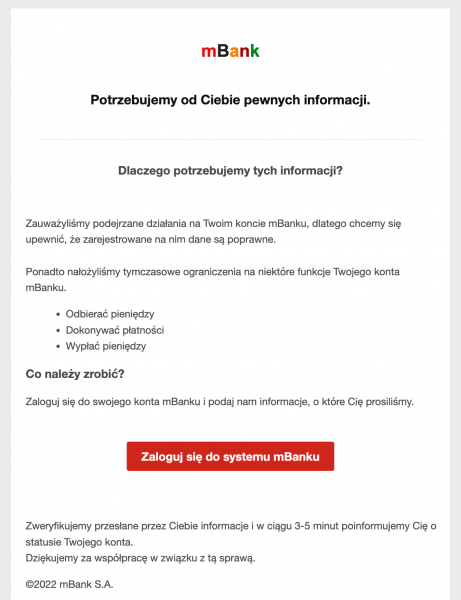
\includegraphics[width=0.6\linewidth]{Pictures/mbank_phishing.png}
	\caption{Przykład ataku typu phishing, Niebezpiecznik.pl, 2022}
	\label{fig:mbankPhishing}
\end{figure}

W przypadku adresów URL ważną kwestią jest jego uważne sprawdzenie litera po literze, ponieważ różnice bywają ciężkie do dostrzeżenia. W pośpiechu może umknąć różnica pomiędzy małym L: "l", a wielkim i: "I". Wielkie "O" może przypominać "0" itd. Trudniejszymi przypadkami są ataki typu \textit{IDN homograph attack}. Ich istota tkwi w tym, że alfabety posiadają litery, które są identyczne, jednakże ich kody \textit{Unicode} się różnią. Dla przykładu alfabety: grecki, cyrylica, łaciński posiadają literę ⟨o⟩, która dla człowieka jest nierozróżnialna \cite{idn_homograph}. "Komputer" z rozróżnianiem liter nie ma najmniejszego problemu, stąd też da się go (a następnie ofiary) łatwo oszukać i zarejestrować domenę bliźniaczą do znanej, zaufanej przez potencjalną ofiarę. Bywa również, że między \textit{hostem} a \textit{subdomeną} brakuje kropki. Jest to znane jako \textit{Doppelganger Domain} \cite{doppelganger}. Należy uważać również na jaką stronę kieruje hiperłącze, ponieważ tekst hiperłącza niekoniecznie musi oznaczać, że jego atrybut \textit{href} służący do wskazywania adresu docelowego - faktycznie wskazuje na pokazany adres.

\begin{figure}[h!]
	\centering
	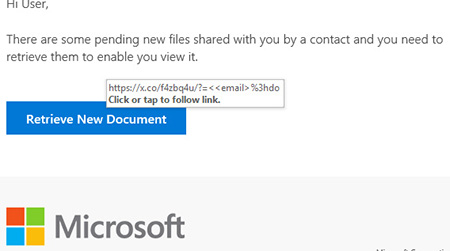
\includegraphics[width=0.6\linewidth]{Pictures/url_phishing.jpg}
	\caption{Przykład fałszywego hiperłącza, digitalcheck.com, 2021}
	\label{fig:url_phishing}
\end{figure}

\section{Rozpoznawanie phishingu przy pomocy nauczania maszynowego}

....
% https://arxiv.org/pdf/2201.10752.pdf
\subsection{Dobór parametrów}
Przy rozpoznawaniu phishingu w wiadomościach e-mail kluczowe jest \textit{body} wiadomości. Naturalnie znajduje się tam najwięcej treści, w tym \textit{odnośniki} i \textit{podpisy}. W oparciu o podejmiemy się utworzenia klasyfikatora, który pod uwagę bierze 10 cech. 

\subsubsection{Certyfikat SSL}
...
Jeżeli HTTPS -> legit
JEŻELI inny -> podejrzany

\subsubsection{Autoryzacja certyfikatu}
Authentic CA -> legit SSL
otherwise -> suspicious

\subsubsection{Czarna lista słów}
"Click Now", "Verify Now," "Valid in 24h", and "Update Now."
email word in {blacklist} -> sus
otherwise -> legit

\subsubsection{Odnośniki przekierowywujące}
GET request of the HTTP protocol is used to verify the legitimacy of an URL.

\subsubsection{Ukrywane odnośniki}
"goo.gl", or "j.mp"

\subsubsection{Adres IP wewnątrz odnośnika}
adres ip w odnośniku -> sus
brak adresu -> legit

\subsubsection{Ruch wewnątrz strony internetowej}
maly ruch -> sus
duzy ruch -> legit

\subsubsection{Wiek strony internetowej}
starsza niz rok -> legit
mlodsza -> sus

\subsubsection{Adres e-mail nadawcy}


\section{Skutki ataków phishingowych}

\newpage
\section{Ochrona przed phishingiem}

\newpage
\section{Studium przypadku: Znane ataki phishingowe}

\newpage
\section{Przyszłość phishingu}

\newpage
\section{Podsumowanie}

\newpage
\bibliographystyle{plain}
\bibliography{bibliografia.bib}
\end{document}
